%\documentclass{jss}
\documentclass[nojss]{jss}
\usepackage[OT1]{fontenc}
%\usepackage[latin1]{inputenc}
\usepackage{graphicx}
\usepackage{amsmath}

%\usepackage{cite}
\usepackage{draftwatermark}
\SetWatermarkText{Draft}
\SetWatermarkScale{1.5}

%\usepackage{myVignette}

%\VignetteIndexEntry{An introduction to markovchain package}
%\VignetteKeywords{vig1}
%\VignettePackage{lifecontingencies}
% need no \usepackage{Sweave.sty}

%\SweaveOpts{prefix.string=Figures/fig}
%%%%%%%%%%%%%%%%%%%%%%%%%%%%%%
%% declarations for jss.cls %%%%%%%%%%%%%%%%%%%%%%%%%%%%%%%%%%%%%%%%%%
%%%%%%%%%%%%%%%%%%%%%%%%%%%%%%

%% almost as usual
\author{Giorgio Alfredo Spedicato, Ph.D C.Stat ACAS}
\title{The \pkg{markovchain} Package: A Package for Easily Handling Discrete
Markov Chains in \proglang{R}}

%% for pretty printing and a nice hypersummary also set:
\Plainauthor{Giorgio Alfredo Spedicato, Ph.D C.Stat ACAS} %% comma-separated
\Plaintitle{The markovchaing Package: A Package for Easily Handling Discrete
Markov Chains in R} %% without formatting
\Shorttitle{The markovchain package} %% a short title (if necessary)
%% an abstract and keywords
\Abstract{\pkg{markovchain} aims to fill a gap within R packages providing S4
classes and methods to easily handling discrete markov chains. The S4 class
structure will be presented as well implemented classes and methods. Applied
examples will follow} \Keywords{markov chain, transition probabilities}
\Plainkeywords{markov chain, transition probabilities} %% without formatting
%% at least one keyword must be supplied

%% publication information
%% NOTE: Typically, this can be left commented and will be filled out by the technical editor
%% \Volume{13}
%% \Issue{9}
%% \Month{September}
%% \Year{2004}
%% \Submitdate{2004-09-29}
%% \Acceptdate{2004-09-29}

%% The address of (at least) one author should be given
%% in the following format:
\Address{
  Giorgio Alfredo Spedicato\\
  StatisticalAdvisor\\
  Via Firenze 11
  20037 Italy\\
  Telephone: +39/334/6634384\\
  E-mail: \email{spedygiorgio@gmail.com}\\
  URL: \url{www.statisticaladvisor.com}
}


%% for those who use Sweave please include the following line (with % symbols):
%% need no \usepackage{Sweave.sty}

%% end of declarations %%%%%%%%%%%%%%%%%%%%%%%%%%%%%%%%%%%%%%%%%%%%%%%

\begin{document}


\maketitle

\section{Introduction}

Markov chains represent a class of stochastic processes of great interest for the wide spectrum of practical applications. %inserire citazione.
In particular, discrete markov chains permit to model the transition probabilities between possible discrete states by the aid of matrices.
Various R packages deals with Markov chains processes and their applications: \pkg{msm} \citep{msmR} works with Multi-State Models for Panel Data, \pkg{mcmcR} \citep{mcmcR} is only one of the many package that implements Monte Carlo Markov Chain approach for estimating models' parameters, \pkg{hmm} fits hidden markov models taking into account covariates. R statistical environments seems to lack a simple R package that coherently defines S4 classes for discrete Markov chains and that allows the statistical analyst to perform probabilistic analysis and statistical infrence.  \pkg{markovchain} \citep{markovchainR} aims to offer greater flexibility in handling discrete time Markov chains. The paper is structured as it follows: Section~\ref{sec:mathematic} briefly revies mathematic and definitions on discrete Markov chains, Section~\ref{sec:examples} shows applied example of discrete Markov chains in various fields.


\section{Markov chains mathematic revies}\label{sec:mathematic}

A general overview of Discrete Markov chains can be found in various web sites. See for example \cite{wiki:markov} and \cite{chapter11}.


\section{The structure of the package}\label{sec:structure}
\subsection{Creating markovchain objects}

The package \pkg{markovchain} contains classes and methods that handle 
markov chain in a convenient manner.\\

The package is loaded within the \proglang{R} command line as follows:

\begin{Schunk}
\begin{Sinput}
R> library("markovchain")
\end{Sinput}
\end{Schunk}



The \code{markovchain} and  \code{markovchainList}  S4 classes \citep(chambers) is defined within the \pkg{markovchain} package as displayed:

\begin{Schunk}
\begin{Soutput}
Class "markovchain" [package "markovchain"]

Slots:
                                                         
Name:            states            byrow transitionMatrix
Class:        character          logical           matrix
                       
Name:              name
Class:        character
\end{Soutput}
\begin{Soutput}
Class "markovchainList" [package "markovchain"]

Slots:
                                
Name:  markovchains         name
Class:         list    character
\end{Soutput}
\end{Schunk}

Any element of \code{markovchain} class is comprised by following slots:
\begin{enumerate}
  \item \code{states}: a character vector, listing the states for which transition probabilities are defined.
  \item \code{byrow}: a logical element, indicating whether transition probabilities are shown by row or by column.
  \item \code{transitionMatrix}: the probabilities of transition matrix.
  \item \code{name}: optional character element to name the Markov chain
\end{enumerate}


\code{markovchain} objects can be created either in a long way, as the following code shows,

\begin{Schunk}
\begin{Sinput}
R> weatherStates<-c("sunny", "cloudy", "rain")
R> byRow<-TRUE
R> weatherMatrix<-matrix(data=c(0.70, 0.2,0.1,
+                         0.3,0.4, 0.3,
+                         0.2,0.45,0.35),byrow=byRow, nrow=3,
+                       dimnames=list(weatherStates, weatherStates))
R> mcWeather<-new("markovchain",states=weatherStates, byrow=byRow, 
+                 transitionMatrix=weatherMatrix, name="Weather")
\end{Sinput}
\end{Schunk}

or in a shorter way, displayed below.

\begin{Schunk}
\begin{Sinput}
R> mcWeather<-new("markovchain", states=c("sunny", "cloudy", "rain"), transitionMatrix=matrix(data=c(0.70, 0.2,0.1,
+                         0.3,0.4, 0.3,
+                         0.2,0.45,0.35),byrow=byRow, nrow=3), name="Weather")
R> 
\end{Sinput}
\end{Schunk}

When \code{new("markovchain")} is called alone a defaut Markov chain is created.

\begin{Schunk}
\begin{Sinput}
R> defaultMc<-new("markovchain")
\end{Sinput}
\end{Schunk}

The quicker form of object creation is made possible thanks to the implemented \code{initialize} S4 method that assures:

\begin{itemize}
  \item the \code{transitionMatrix} to be a transition matrix, i.e., all entries to be probabilities and either all rows or all columns to sum up to one, according to the value of \code{byrow} slot.
  \item the columns and rows nams of \code{transitionMatrix} to be defined and to coincide with \code{states} vector slot. 
\end{itemize}

\code{markovchain} objects can be collected in a list within \code{markovchainList} S4 objects as following example shows.

\begin{Schunk}
\begin{Sinput}
R> mcList<-new("markovchainList",markovchains=list(mcWeather, defaultMc), name="A list of Markov chains")
\end{Sinput}
\end{Schunk}



\subsection{Handling markovchain objects}

\pkg{markovchain} contains two classes, \code{markovchain} and \code{markovchainList}. \code{markovchain} objects handle discrete Markov chains, whilst \code{markovchainList} objects consists in list of \code{markovchain} that can be useful to model non - homogeneous Markov chain processess.\\

Following methods have been implemented within the package for \code{markovchain} and \code{markovchainLists} respectively:

\begin{Schunk}
\begin{Soutput}
Function: * (package base)
e1="markovchain", e2="markovchain"
e1="markovchain", e2="matrix"
e1="markovchain", e2="numeric"
e1="matrix", e2="markovchain"
e1="numeric", e2="markovchain"

Function: ^ (package base)
e1="markovchain", e2="numeric"

Function: == (package base)
e1="markovchain", e2="markovchain"

Function: absorbingStates (package markovchain)
object="markovchain"

Function: coerce (package methods)
from="data.frame", to="markovchain"
from="markovchain", to="data.frame"

Function: dim (package base)
x="markovchain"

Function: initialize (package methods)
.Object="markovchain"


Function "isDiagonal":
 <not an S4 generic function>

Function "isTriangular":
 <not an S4 generic function>
Function: plotMc (package markovchain)
object="markovchain"

Function: print (package base)
x="markovchain"

Function: show (package methods)
object="markovchain"

Function: states (package markovchain)
object="markovchain"

Function: steadyStates (package markovchain)
object="markovchain"

Function: t (package base)
x="markovchain"

Function: transitionProbability (package markovchain)
object="markovchain"
\end{Soutput}
\begin{Soutput}
Function: initialize (package methods)
.Object="markovchainList"
    (inherited from: .Object="ANY")


Function "isDiagonal":
 <not an S4 generic function>

Function "isTriangular":
 <not an S4 generic function>
\end{Soutput}
\end{Schunk}

Table~\ref{tab:methodsToHandle} lists which of implemented methods handle and manipulate \code{markovchain} objects.



\begin{table}[h]
  \centering
  \begin{tabular}{lll}
    \hline
  Method & Purpose \\
    \hline  \hline

  * & Algebraic operators on the transition matrix.\\
  \code{==} & Equality operator on the transition matrix.\\
\code{dim} & Dimenion of the transition matrix.\\
  \code{states} & Defined transition states.\\
  \code{t} & Transposition operator (it switches byrow slot value and modifies the transition matrix coherently).\\
  \code{as} & Operator con switch from \code{markovchain} objects to \code{data.frame} objects and vice - versa.\\
  \hline
\end{tabular}
\caption{\pkg{markovchain} methods: matrix handling.}
\label{tab:methodsToHandle}
\end{table}  

Operations on the markovchains objects can be easily performed.
Using the previously defined matrix we can find what is the probability distribution of expected weather states two and  seven days after, given actual state to be cloudy. 

\begin{Schunk}
\begin{Sinput}
R> initialState<-c(0,1,0)
R> after2Days<-initialState*(mcWeather*mcWeather)
R> after7Days<-initialState*(mcWeather^7)
R> after2Days
\end{Sinput}
\begin{Soutput}
     sunny cloudy  rain
[1,]  0.39  0.355 0.255
\end{Soutput}
\begin{Sinput}
R> after7Days
\end{Sinput}
\begin{Soutput}
         sunny    cloudy      rain
[1,] 0.4622776 0.3188612 0.2188612
\end{Soutput}
\end{Schunk}

A similar answer could have been obtained if the probabilities were defined by 
column. A column - defined probability matrix could be set up either creating a new matrix or transposing an existing \code{markovchain} object thanks to the \code{t} vector.

\begin{Schunk}
\begin{Sinput}
R> initialState<-c(0,1,0)
R> mcWeatherTransposed<-t(mcWeather)
R> after2Days<-(mcWeatherTransposed*mcWeatherTransposed)*initialState
R> after7Days<-(mcWeather^7)*initialState
R> after2Days
\end{Sinput}
\begin{Soutput}
        [,1]
sunny  0.390
cloudy 0.355
rain   0.255
\end{Soutput}
\begin{Sinput}
R> after7Days
\end{Sinput}
\begin{Soutput}
            [,1]
sunny  0.3172005
cloudy 0.3188612
rain   0.3192764
\end{Soutput}
\end{Schunk}

Basing informational methods have been defined for \code{markovchain} objects to quickly get states and dimension.

\begin{Schunk}
\begin{Sinput}
R> states(mcWeather)
\end{Sinput}
\begin{Soutput}
[1] "sunny"  "cloudy" "rain"  
\end{Soutput}
\begin{Sinput}
R> dim(mcWeather)
\end{Sinput}
\begin{Soutput}
[1] 3
\end{Soutput}
\end{Schunk}

A direct access to transition probabilities is provided by \code{transitionProbability} method.

\begin{Schunk}
\begin{Sinput}
R> transitionProbability(mcWeather, "cloudy","rain")
\end{Sinput}
\begin{Soutput}
[1] 0.3
\end{Soutput}
\end{Schunk}

A transition matrix can be displayed using \code{print}, \code{show} methods (the latter being less laconic). Similarly, the underlying transition probability diagram can be plot by the use of \code{plotMc} method that was based on \pkg{igraph} package \citep{pkg:igraph} as Figure~\ref{fig:mcPlot} displays.

\begin{Schunk}
\begin{Sinput}
R> print(mcWeather)
\end{Sinput}
\begin{Soutput}
       sunny cloudy rain
sunny    0.7   0.20 0.10
cloudy   0.3   0.40 0.30
rain     0.2   0.45 0.35
\end{Soutput}
\begin{Sinput}
R> show(mcWeather)
\end{Sinput}
\begin{Soutput}
Weather 
 A  3 - dimensional discrete Markov Chain with following states 
 sunny cloudy rain 
 The transition matrix   (by rows)  is defined as follows 
       sunny cloudy rain
sunny    0.7   0.20 0.10
cloudy   0.3   0.40 0.30
rain     0.2   0.45 0.35
\end{Soutput}
\end{Schunk}

\begin{figure}
\begin{center}
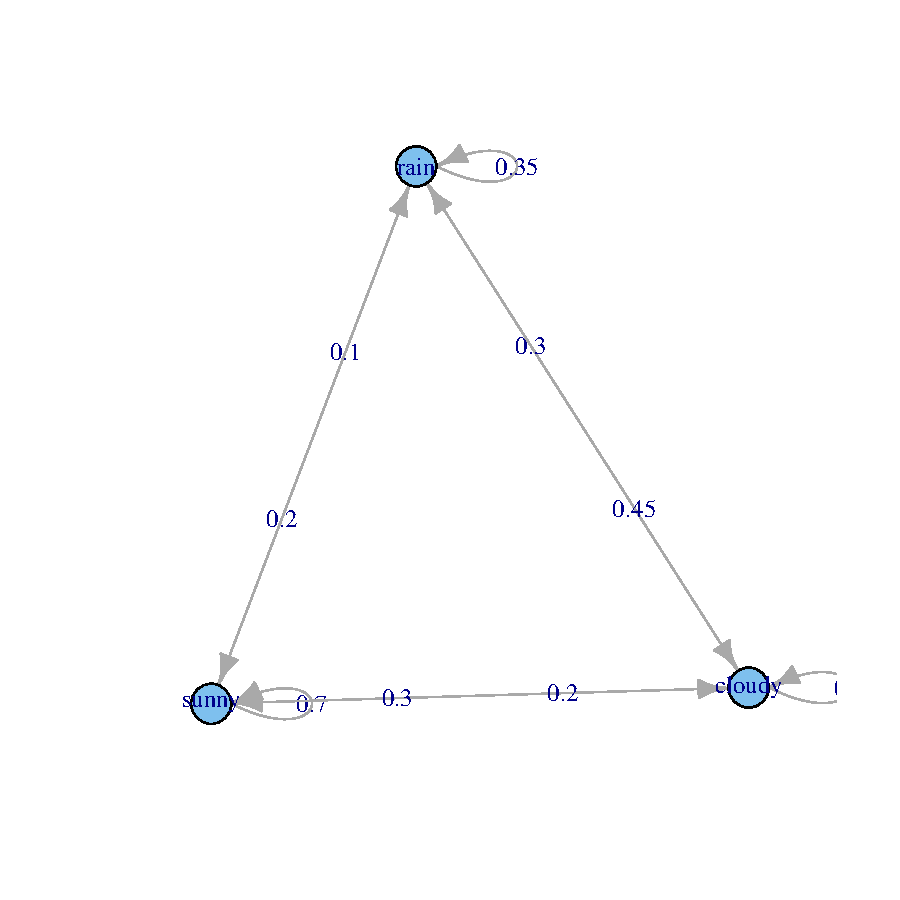
\includegraphics{an_introduction_to_markovchain_package-mcPlot}
\caption{Weather example Markov chain plot}
\label{fig:mcPlot}
\end{center}
\end{figure}

The \pkg{igraph} package \citep{pkg:igraph} is used for plotting. \code{...} additional parameters are passed to \code{graph.adjacency} function to control the graph layout.

Exporting to \code{data.frame} is possible and similarly it is possible to import.

\begin{Schunk}
\begin{Sinput}
R> mcDf<-as(mcWeather, "data.frame")
R> mcNew<-as(mcDf, "markovchain")
\end{Sinput}
\end{Schunk}

Similarly it is possible to export a \code{markovchain} class toward an adjacency matrix.

\subsection{Statistics with markovchain objects}

Table~\ref{tab:methodsToStats} shows methods appliable on \code{markovchain} objects to perform probabilistic analysis. 

\begin{table}[h]
  \centering
  \begin{tabular}{lll}
    \hline
  Method & Purpose \\
    \hline  \hline
  \code{absorbingStates} & it returns the absorbing states of the transition matrix, if any.\\
  \code{steadyStates} & it returns the vector(s) of steady state(s) in matricial form.\\
\hline
\end{tabular}
\caption{\pkg{markovchain} methods: statistical operations.}
\label{tab:methodsToStats}
\end{table}

The steady state(s), also known as stationary distribution(s),  of the Markov chains are identified by the following algorithm:
\begin{enumerate}
  \item decompose the Markov Chain in eigenvalues and eigenvectors.
  \item consider only eigenvectors corresponding to eigenvalues equal to one.
  \item normalize such eigenvalues so the sum of their components to total one.
\end{enumerate}

The result is returned in matricial form.

\begin{Schunk}
\begin{Sinput}
R> steadyStates(mcWeather)
\end{Sinput}
\begin{Soutput}
         sunny    cloudy      rain
[1,] 0.4636364 0.3181818 0.2181818
\end{Soutput}
\end{Schunk}

It is possible a Markov chain to have more than one stationary distribuition, as the gambler ruin example shows.

\begin{Schunk}
\begin{Sinput}
R> gamblerRuinMarkovChain<-function(moneyMax, prob=0.5) {
+    require(matlab)
+    matr<-zeros(moneyMax+1)
+    states<-as.character(seq(from=0, to=moneyMax, by=1))
+    rownames(matr)=states; colnames(matr)=states
+    matr[1,1]=1;matr[moneyMax+1,moneyMax+1]=1
+    for(i in 2:moneyMax)
+    {
+      matr[i,i-1]=1-prob;matr[i,i+1]=prob
+    }
+    out<-new("markovchain",  
+             transitionMatrix=matr, 
+             name=paste("Gambler ruin",moneyMax,"dim",sep=" ")
+             )
+    return(out)
+  }
R> mcGR4<-gamblerRuinMarkovChain(moneyMax=4, prob=0.5)
R> steadyStates(mcGR4)
\end{Sinput}
\begin{Soutput}
     0 1 2 3 4
[1,] 1 0 0 0 0
[2,] 0 0 0 0 1
\end{Soutput}
\end{Schunk}

Any absorbing state is determined by the inspection of results returned by \code{steadyStates} method.

\begin{Schunk}
\begin{Sinput}
R> absorbingStates(mcGR4)
\end{Sinput}
\begin{Soutput}
[1] "0" "4"
\end{Soutput}
\begin{Sinput}
R> absorbingStates(mcWeather)
\end{Sinput}
\begin{Soutput}
character(0)
\end{Soutput}
\end{Schunk}

Table~\ref{tab:packageFuns} lists functions (and their purpose) as implemented within the package that helps to fit and simulate discrete time Markov chains.

\begin{table}[h]
  \centering
  \begin{tabular}{lll}
    \hline
  Function & Purpose \\
    \hline  \hline
  \code{markovchainFit} & function to return fitten markov chain for a given sequence.\\
  \code{markovchainSequence} & function to obtain a sample of the stationary process underlying the markov chain.\\
    \hline
\end{tabular}
\caption{\pkg{markovchain} statistical functions.}
\label{tab:packageFuns}
\end{table}  


Simulating a random sequence from an underlying Markov chain is quite easy thanks to the function \code{markovchainSequence}.
The following code generates a "year" of weather states according to \cite{mcWeather} underlying markovian stochastic process.

\begin{Schunk}
\begin{Sinput}
R> weathersOfDays<-markovchainSequence(n=365,markovchain=mcWeather,t0="sunny")
R> weathersOfDays[1:20]
\end{Sinput}
\begin{Soutput}
 [1] "sunny"  "cloudy" "cloudy" "cloudy" "sunny"  "cloudy" "cloudy"
 [8] "cloudy" "cloudy" "cloudy" "cloudy" "cloudy" "sunny"  "sunny" 
[15] "sunny"  "sunny"  "sunny"  "sunny"  "cloudy" "rain"  
\end{Soutput}
\end{Schunk}

Similarly, a \code{markovchain} object can be fit from given data

\begin{Schunk}
\begin{Sinput}
R> mcFitted<-markovchainFit(data=weathersOfDays, method="mle")
\end{Sinput}
\end{Schunk}


\section{Applied examples}\label{sec:examples}

\subsection{Actuarial examples}

Markov chains are widely applied in the fields of actuarial science. Actuaries quantify the risk inherent in insurance contracts evaluating the premium of insurance contract to be sold (therefore covering future risk) and evaluating the actuarial reseves of existing portfolios (the liabilities in terms of benefits or claims payments due to policyholder arising from previously sold contracts).\\
Key quantities of actuarial interest are: the expected present value of future benefits, $PVFB$, the (periodic) benefit premium, $P$, and the present value of future premium $PVFP$. A level benefit premium could be set equating at the beginning of the contract $PVFB=PVFP$. After the beginning of the contract the benefit reserve is the differenbe between $PVFB$ and $PVFP$.
The first example shows the pricing and reserving of a (simple) health insurance contract. The second example analyze the evolution of a MTPL portfolio characterized by Bonus Malus experience rating feature.

\subsubsection{Health insurance example}

The example comes from \cite{deshmukh2012multiple}. The interest rate is 5\%, benefits are payable upon death (1000) and disability (500). Premiums are payable at the beginning of period only if policyholder is active. The contract term is three years 

\begin{Schunk}
\begin{Sinput}
R> mcHI=new("markovchain", states=c("active", "disable", "withdrawn", "death"),
+           transitionMatrix=matrix(c(0.5,.25,.15,.1,
+                                     0.4,0.4,0.0,.2,
+                                     0,0,1,0,
+                                     0,0,0,1), byrow=TRUE, nrow=4))
R> benefitVector=as.matrix(c(0,0,500,1000))
R> 
\end{Sinput}
\end{Schunk}

The policyholders is active at $T_0$. Therefore the expected states at $T_1, \ldots T_3$ are calculated as shown.

\begin{Schunk}
\begin{Sinput}
R> T0=t(as.matrix(c(1,0,0,0)))
R> T1=T0*mcHI
R> T2=T1*mcHI
R> T3=T2*mcHI
\end{Sinput}
\end{Schunk}

Therefore the present value of future benefit at T0 is

\begin{Schunk}
\begin{Sinput}
R> PVFB=T0%*%benefitVector*1.05^-0+T1%*%benefitVector*1.05^-1+T2%*%benefitVector*1.05^-2+T3%*%benefitVector*1.05^-3
\end{Sinput}
\end{Schunk}

and the yearly premium payable whether the insured is alive is 

\begin{Schunk}
\begin{Sinput}
R> P=PVFB/(T0[1]*1.05^-0+T1[1]*1.05^-1+T2[1]*1.05^-2)
\end{Sinput}
\end{Schunk}

The reserve at the beginning of year two, in case of the insured being alive, is

\begin{Schunk}
\begin{Sinput}
R> PVFB=(T2%*%benefitVector*1.05^-1+T3%*%benefitVector*1.05^-2)
R> PVFP=P*(T1[1]*1.05^-0+T2[1]*1.05^-1)
R> V=PVFB-PVFP
R> V
\end{Sinput}
\begin{Soutput}
         [,1]
[1,] 300.2528
\end{Soutput}
\end{Schunk}


\section{Aknowledgments}\label{sec:aknowledgements}



\bibliography{markovchainBiblio}



\end{document}
